
\documentclass[notheorems,serif]{beamer}

%选用主题
%\usetheme{Rochester}
%\usetheme{default}
%\usetheme{AnnArbor}
%\usetheme{Antibes}
%\usetheme{Bergen}
%\usetheme{Berkeley}
%\usetheme{Berlin}
%\usetheme{Boadilla}
%\usetheme{CambridgeUS}
%\usetheme{Copenhagen}
%\usetheme{Darmstadt}
%\usetheme{Dresden}
%\usetheme{Frankfurt}
%\usetheme{Goettingen}
%\usetheme{Hannover}
%\usetheme{Ilmenau}
%\usetheme{JuanLesPins}
%\usetheme{Luebeck}
\usetheme{Madrid}
%\usetheme{Malmoe}
%\usetheme{Marburg}
%\usetheme{Montpellier}
%\usetheme{PaloAlto}
%\usetheme{Pittsburgh}
%\usetheme{Rochester}
%\usetheme{Singapore}
%\usetheme{Szeged}
%\usetheme{Warsaw}

% As well as themes, the Beamer class has a number of color themes
% for any slide theme. Uncomment each of these in turn to see how it
% changes the colors of your current slide theme.

%\usecolortheme{albatross}
%\usecolortheme{beaver}
%\usecolortheme{beetle}
%\usecolortheme{crane}
%\usecolortheme{dolphin}
%\usecolortheme{dove}
%\usecolortheme{fly}
%\usecolortheme{lily}
%\usecolortheme{orchid}
%\usecolortheme{rose}
%\usecolortheme{seagull}
%\usecolortheme{seahorse}
%\usecolortheme{whale}
%\usecolortheme{wolverine}

%设置被cover的内容不显示
%\setbeamercovered{transparent}

\useinnertheme{rounded}
\usecolortheme{default}

%调用包
\usepackage[no-math, cm-default]{fontspec}
\usepackage{xltxtra}
\usepackage{xunicode}   
\usepackage{xcolor}
\usepackage{amsmath,amssymb}
\usepackage{xeCJK}
\usepackage{multimedia}
\usepackage{listings}
\usepackage{subfigure}
\usepackage{todonotes}
\presetkeys{todonotes}{inline}{} 
\usepackage{multicol}
\usepackage{changes}



%将系统字体名映射为逻辑字体名称,主要是为了维护的方便  
\newcommand\fnhei{Adobe 黑体 Std}  
\newcommand\fnsong{Adobe 宋体 Std}  
\newcommand\fnkai{Adobe 楷体 Std}  
\newcommand\fnmono{DejaVu Sans Mono}  
\newcommand\fnroman{Times New Roman}  

\renewcommand{\normalsize}{\wuhao}

%%设置常用中文字号,方便调用  
\newcommand{\erhao}{\fontsize{22pt}{\baselineskip}\selectfont}  
\newcommand{\xiaoerhao}{\fontsize{18pt}{\baselineskip}\selectfont}  
\newcommand{\sanhao}{\fontsize{16pt}{\baselineskip}\selectfont}  
\newcommand{\xiaosanhao}{\fontsize{15pt}{\baselineskip}\selectfont}  
\newcommand{\sihao}{\fontsize{14pt}{\baselineskip}\selectfont}  
\newcommand{\xiaosihao}{\fontsize{12pt}{\baselineskip}\selectfont}  
\newcommand{\wuhao}{\fontsize{10.5pt}{\baselineskip}\selectfont}  
\newcommand{\xiaowuhao}{\fontsize{9pt}{\baselineskip}\selectfont}  
\newcommand{\liuhao}{\fontsize{7.5pt}{\baselineskip}\selectfont}  

%\setmainfont{\fnroman}
\setmainfont{\fnkai}
\setCJKmainfont[BoldFont=\fnhei]{\fnkai}  
\setCJKsansfont[BoldFont=\fnhei]{\fnkai}  
\setCJKmonofont{\fnkai}  

%楷体  
%\newfontinstance\KAI{\fnkai}  
%\newcommand{\kai}[1]{{\KAI#1}}  
%黑体  
%\newfontinstance\HEI{\fnhei}  
%\newcommand{\hei}[1]{{\HEI#1}}  
%英文  
%\newfontinstance\ENF{\fnroman}  
%\newcommand{\en}[1]{\,{\ENF#1}\,}

%楷体  
\newfontfamily\KAI {\fnkai}  
\newcommand{\kai}[1]{{\KAI#1}}  
%黑体  
\newfontfamily\HEI{\fnhei}  
\newcommand{\hei}[1]{{\HEI#1}}  
%英文  
\newfontfamily\ENF{\fnroman}  
\newcommand{\en}[1]{\,{\ENF#1}\,}


%连字符
\defaultfontfeatures{Mapping=tex-text}

%中文断行
\XeTeXlinebreaklocale "zh"
\XeTeXlinebreakskip = 0pt plus 1pt minus 0.1pt


%%%% 定理类环境的定义 %%%%
\newtheorem{example}{\hei{例子}} 
\newtheorem{problem}{\hei{问题}}           
\newtheorem{algorithm}{\hei{算法}}
\newtheorem{theorem}{\hei{定理}}
\newtheorem{definition}{\hei{定义}}
\newtheorem{axiom}{\hei{公理}}
\newtheorem{property}{\hei{性质}}
\newtheorem{proposition}{\hei{命题}}
\newtheorem{lemma}{\hei{引理}}
\newtheorem{corollary}{\hei{推论}}
\newtheorem{remark}{\hei{注解}}
\newtheorem{condition}{\hei{条件}}
\newtheorem{conclusion}{\hei{结论}}
\newtheorem{assumption}{\hei{假设}}

%重定义一些环境的名字
\renewcommand{\proofname}{\hei{证明}}
\renewcommand\tablename{\hei{表}}

%---SCRIPT-----------------------------------------------------------------------------------------
\newcommand{\cA}{\mathcal{A}}
\newcommand{\cB}{\mathcal{B}}
\newcommand{\cC}{\mathcal{C}}
\newcommand{\cD}{\mathcal{D}}
\newcommand{\cE}{\mathcal{E}}
\newcommand{\ce}{\mathcal{e}}
\newcommand{\cF}{\mathcal{F}}
\newcommand{\cG}{\mathcal{G}}
\newcommand{\cg}{\mathcal{g}}
\newcommand{\cH}{\mathcal{H}}
\newcommand{\cI}{\mathcal{I}}
\newcommand{\cJ}{\mathcal{J}}
\newcommand{\cK}{\mathcal{K}}
\newcommand{\cL}{\mathcal{L}}
\newcommand{\cM}{\mathcal{M}}
\newcommand{\cN}{\mathcal{N}}
\newcommand{\cO}{\mathcal{O}}
\newcommand{\cP}{\mathcal{P}}
\newcommand{\cQ}{\mathcal{Q}}
\newcommand{\cR}{\mathcal{R}}
\newcommand{\cS}{\mathcal{S}}
\newcommand{\cT}{\mathcal{T}}
\newcommand{\cU}{\mathcal{U}}
\newcommand{\cV}{\mathcal{V}}
\newcommand{\cW}{\mathcal{W}}
\newcommand{\cX}{\mathcal{X}}
\newcommand{\cY}{\mathcal{Y}}
\newcommand{\cZ}{\mathcal{Z}}
\newcommand{\cz}{\mathcal{z}}
%---BLACKBOARD-------------------------------------------------------------------------------------
\newcommand{\mA}{\mathbb A}
\newcommand{\mB}{\mathbb B}
\newcommand{\mC}{\mathbb C}
\newcommand{\mD}{\mathbb D}
\newcommand{\mE}{\mathbb E}
\newcommand{\mF}{\mathbb F}
\newcommand{\mG}{\mathbb G}
\newcommand{\mg}{\mathbb g}
\newcommand{\mH}{\mathbb H}
\newcommand{\mI}{\mathbb I}
\newcommand{\mJ}{\mathbb J}
\newcommand{\mK}{\mathbb K}
\newcommand{\mL}{\mathbb L}
\newcommand{\mM}{\mathbb M}
\newcommand{\mN}{\mathbb N}
\newcommand{\mO}{\mathbb O}
\newcommand{\mP}{\mathbb P}
\newcommand{\mQ}{\mathbb Q}
\newcommand{\mR}{\mathbb R}
\newcommand{\mS}{\mathbb S}
\newcommand{\mT}{\mathbb T}
\newcommand{\mU}{\mathbb U}
\newcommand{\mV}{\mathbb V}
\newcommand{\mW}{\mathbb W}
\newcommand{\mX}{\mathbb X}
\newcommand{\mY}{\mathbb Y}
\newcommand{\mZ}{\mathbb Z}
\newcommand{\mz}{\mathbb z}

\newcommand{\bV}{\mathbf{V}}
\newcommand{\bz}{\mathbf{z}}
\newcommand{\bT}{\mathbf{T}}
\newcommand{\bx}{\mathbf{x}}
\newcommand{\be}{\mathbf{e}}
\newcommand{\bff}{\mathbf{f}}
\newcommand{\bg}{\mathbf{g}}
\newcommand{\bn}{\mathbf{n}}
\newcommand{\bt}{\mathbf{t}}
\newcommand{\bd}{\mathbf{d}}
\newcommand{\bzero}{\mathbf{0}}
\newcommand{\bka}{\mathbf{\kappa}}

\newcommand{\rd}{\mathrm{d}}
%---SHORTCUTS--------------------------------------------------------------------------------------
\newcommand\xor{\mathbin{\char`\^}}
\DeclareMathOperator{\res}{Res}
\DeclareMathOperator{\sgn}{sgn}
\DeclareMathOperator{\supp}{supp}
\DeclareMathOperator{\as}{as}
\newcommand{\slant}[1]{\slshape #1\normalfont}
\newcommand{\dd}[2]{\frac{d#1}{d#2}} 
\newcommand{\ddx}{\frac{d}{dx}}
\newcommand{\ddt}{\frac{d}{dt}}
\newcommand{\dds}{\frac{d}{ds}}
\newcommand{\pd}[1]{\ds\frac{\partial}{\partial #1 }}
\newcommand{\pdd}[2]{\ds\frac{\partial #1}{\partial #2 }}
\newcommand{\mdd}[3]{\ds\frac{\partial^{#3} #1}{\partial #2^{#3} }}
\newcommand{\x}{\ _\Box}
\newcommand{\ds}{\displaystyle}
\newcommand{\bs}{\backslash}
\newcommand{\Bold}{\noindent \bfseries}
\newcommand{\Norm}{\normalfont}
\newcommand{\exl}[1]{\textcolor{NavyBlue}{\Bold Exercise #1 \Norm}}
\newcommand{\ex}{\textcolor{NavyBlue}{\Bold Problem: \Norm}}
\newcommand{\sol}{\textcolor{Mulberry}{\Bold Solution: \Norm}}
\newcommand{\pf}{\textcolor{Mulberry}{\Bold Proof: \Norm}}
\newcommand{\Title}[1]{\LARGE\Bold \textcolor{Sepia}{#1}\Norm\normalsize \vspace{10pt} \newline}
\newcommand{\prop}{\Bold \textcolor{YellowOrange}{ Proposition:} \Norm}
\newcommand{\propl}[1]{\Bold \textcolor{YellowOrange}{ Proposition #1:} \Norm}
\newcommand{\rk}{\Bold \textcolor{YellowOrange}{ Remark:} \Norm}
\newcommand{\rmk}[1]{\Bold\textcolor{YellowOrange}{#1} \Norm}
\newcommand{\thm}[1]{\Bold \textcolor{YellowOrange}{ Theorem #1} \Norm}
\newcommand{\ind}{\indent\indent}
\newcommand{\br}{\vspace{10pt} \newline}

\newcommand{\red}{\color{red}}
\newcommand{\blue}{\color{blue}}



\begin{document}

\title[湘潭大学硕士研究生开题报告]{{\small \leftline{湘潭大学硕士研究生开题报告}~~~~~~~~~~~~~~~~~~~~~~~~~~~~~~~~~~~~~~~~~~~~~~
~~~~~~~~~~~} \\
\leftline{基于有限元方法的一般曲面上的自洽场理论的数值模拟}
}




\author[许明]{~~~报告人:~~许~~明~~ \\
\vspace{0.2cm}
		~~~专~~~~业:~~数~~学~~\\
\vspace{0.2cm}
              \qquad\qquad\qquad ~~导~~~~师:~~魏华祎、蒋凯 ~副教授\\
                }

\institute[湘潭大学数学与计算科学学院 ]

\date[\today]



\pgfdeclareimage[height=1cm]{institution-logo}{figures/xtu.pdf}

\logo{\pgfuseimage{institution-logo}}


\frame[plain]{\titlepage}


\AtBeginSection[]{

  \frame<beamer>{ 

    \frametitle{内容纲要}   

    \tableofcontents[currentsection] 

  }
}
\section{研究背景及现状}

\begin{frame}
    \frametitle{研究背景}
%
%~~~~ 几何学在许多科学领域起着关键作用, 包括哈密顿力学、广义相对论、量子力
%学、量子场论、球体上电子排列 (汤姆逊问题)、曲面的缺陷运动、聚合物场论,
%    它们通常发生在化学和生物的反应扩散模型. 

~~~~ 自组装是近几十年最为活跃的科学领域之一, 它是形成蛋白质乃至细胞生命的
一个重要领域. 分子自组装是指分子通过共价键相互作用自发组合形成的一类结构明确、
稳定,同时具有某种特定功能或者性能的分子聚集体或超分子结构.

~~~~ 近年来, 在曲面上各种几何限制, 嵌段共聚物的微相分离已经引起了极大的关注, 当适应各种类型的几何限制时,
许多新颖的嵌段共聚物的图案从传统的有序相的重新排列中出现.  


~~~~ 嵌段共聚物在纳米尺度范围内有丰富的自组织现象,形成微观相分离,这使得他们在纳米材料科学例如芯片制造上也有广阔的应用
前景. 例如,高效数据存储器件, 波导,量子点阵列, 电解质镜, 纳米多孔膜和纳米线, 干涉光刻等.

\end{frame}

\begin{frame}
    \frametitle{研究现状}

~~~~ 在过去的 30 年中, 已经提出了两类离散化方案来离散 SCFT 方程:
    \begin{itemize}
        \item 投影空间离散化方法:
            通过给出微观相分离中的嵌段聚合物的相结构以及它的对称群,SCFT方程可以被一组对称的基函数展开. 典型的代表之一是
            Masten and Schick 1994  年提出的投影傅里叶方法. 

        \item 全空间离散化方法: 在实空间和傅里叶空间中进行, 也已经证明了全空间离散化方法能够获得新的结构, 拟谱法被引进解决 SCFT 中的 PDE. 
            它充分利用了实空间和傅里叶空间的最佳优点, 降低了计算复杂度.
    \end{itemize}

    
\end{frame}

\begin{frame}
    \frametitle{研究现状}
    ~~~~ \textbf{前人的工作}
    \begin{itemize}
        \item 2006 年 J. F. Li 等人,模拟了有体积的过程,开发了一个 ADI 格式,在球面上研究了 SCFT.
        \item 2007 年 Tanya L. Chantawansri 等人, 使用球调和方法在球面上研究了 SCFT.
        \item 2014 年 J. F. Li 等人, 模拟了有限体积的过程, 并开发了一个扩展球面的 ADI 有限差分来求解一般曲面上的 SCFT.
        \item 2014 年 Daming Li 等人,使用了拟谱法在环面和圆柱面上的研究了 SCFT.
    \end{itemize}
~~~~ 目前在全空间下的 SCFT 已经做了大量的工作, 但是在曲面上的自组装研究理论不是很多, 没有一个系统的理论框架.
\end{frame}
\section{研究内容及方案}

\begin{frame}
    \frametitle{研究内容}
~~~~ 在全空间下的自组装也就是没有受到几何约束的组装,目前已经有了很多的自组装结构,如下图

\begin{columns}

        \column{6cm}

    \begin{figure}
        \centering
        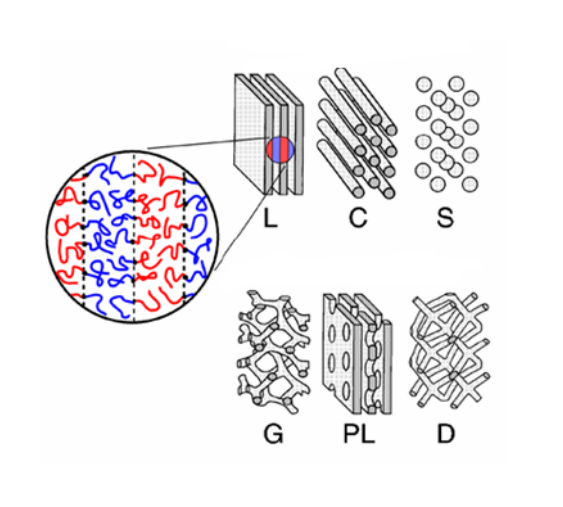
\includegraphics[scale=0.30]{figures/mesh/scft-AB.png}
    \end{figure}
\column{8cm}
    \begin{itemize}
        \item 层状相(Lamellar)
        \item 柱状相(Cylinder)
        \item 球状相(Sphere)
        \item 螺旋相(Gyroid)
        \item 穿孔层状相(Perforated-lamellar)
        \item 双钻相(Double-diamond) 
    \end{itemize}
\end{columns}
~~~~ 我们主要研究带有几何约束的自组装问题, 更具体的而言, 也就是在曲面上的自组装研究. 
\end{frame}

\begin{frame}
    \frametitle{两嵌段共聚物体系}
~~~~ 高分子是由一些单体连接而成的长链分子,这里我们考虑的是由 A-B 两种单体组成的共聚, 也叫两嵌段共聚物,    
\begin{figure}[H]
\centering
\subfigure[]{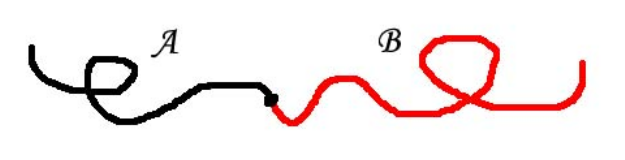
\includegraphics[scale=0.23]{figures/mesh/diblock-AB.png}}
\subfigure[]{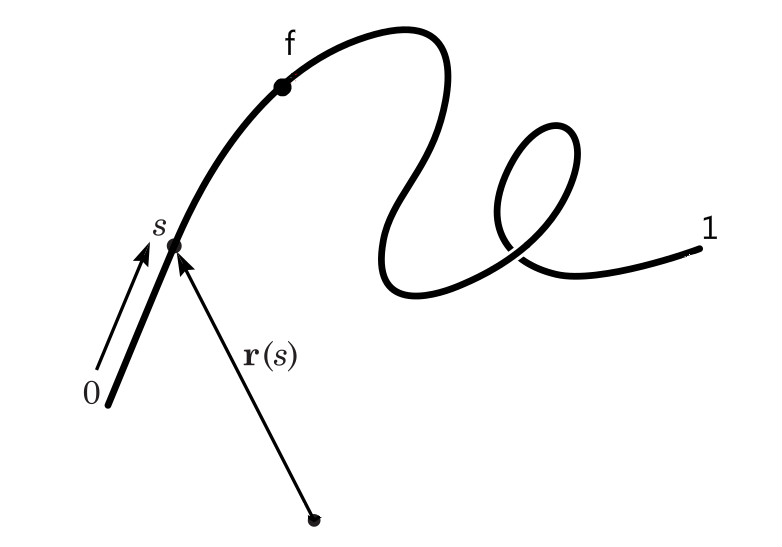
\includegraphics[scale=0.20]{figures/mesh/qplus.jpg}}
\caption{(a) 两嵌段共聚物示意图, (b) 连续高斯链模型示意图.}
\end{figure}
\end{frame}


\begin{frame}
    \frametitle{一般曲面上的自洽场模型}

~~~~ 根据平均场近似, 哈密顿量为:
\begin{tiny}
\begin{equation}
        \begin{aligned}
          H[w_+, w_-] = &
  \frac{1}{S}\int d x\, \left\{ 
  -w_+(x) + \frac{w_-^2(x)}{\chi N} 
        \right\} -\log Q[w_+(x), w_-(x)]
        \label{eq:hamiltonian}
    \end{aligned}
\end{equation}
\end{tiny}

~~~~ 一阶变分,得到 SCFT 方程
\begin{tiny}
    \begin{align}
	& \frac{\delta H}{\delta w_+(x)} = \phi_A(x) + \phi_B(x) - 1 = 0,
	\label{eq:scftwplus}
	\\
	& \frac{\delta H}{\delta w_-(x)} = 
   \frac{2 w_-(x)}{\chi N} - [\phi_A(x) - \phi_B(x)] = 0.
	\label{eq:scftwminus}
    \end{align}
\end{tiny}
~~~~ 结合连续的高斯链完备 SCFT 系统

\begin{tiny}
\begin{columns}
        \column{6cm}
    \begin{align}
  & Q = \frac{1}{S}\int
    d x\,q(x,s)q^\dag(x,s), ~~~ \forall s\in[0,1]
    \label{eq:scft:Q}
  \\
  & \phi_A(x) =
  \frac{1}{Q}\int_0^f ds\,q(x,s)q^{\dag}(x,s),
  \label{eq:scft:phiA}
  \\
  & \phi_B(x) =
  \frac{1}{Q}\int_f^1 ds\,q(x,s)q^{\dag}(x,s).
  \label{eq:scft:phiB}
\end{align}
    \column{6cm}
\begin{equation}
  \label{eq:MDE}
	\begin{aligned}
  \frac{\partial }{\partial s}q(x,s) &=
        \added{\Delta_S} q(x, s) - w(x,s) q(x,s), 
	\\
  q(x,0) &= 1,
  \\
    \frac{\partial }{\partial s}q^\dag(x,s) &=
        - \added{\Delta_S} q^\dag(x, s) + w(x,s)q^\dag(x,s), 
	\\
  q^\dag(x,1) &= 1,
    \\
    w(x,s) &= \left\{   
	\begin{array}{rl}
		w_+(x)-w_-(x), &  0\leq s \leq f,
		\\
		w_+(x) +w_-(x), &  f\leq s \leq 1,
	\end{array}
\right.
	\end{aligned}
\end{equation}
    \end{columns}
\end{tiny}
\end{frame}

\begin{frame}
    \frametitle{研究方案}
~~~~数值求解 SCFT 方程包括以下几个方面

    \begin{itemize}
	\item 初值;
        \item 离散化方案 (主要用于偏微分方程);
	\item 寻求场的鞍点的非线性迭代方法.
    \end{itemize}

\vspace{0.5cm}
~~~~因为 SCFT 是一个非常复杂的变分问题, 具有鞍点优化, 非线性, 多解和多参数等许多不尽人意的特点, 分析解决这个问题超越目前的技术, 这里我们采用曲面线性有限元方法求解 PDE 和 交替迭代的数值方法.

\end{frame}

\section{工作进展及存在的问题}

\begin{frame}
    \frametitle{工作进展}
    \begin{itemize}
        \item 目前已经查找和阅读了一些有关曲面有限元和 SCFT 共聚物自组装的文献;
        \item 对曲面有限元方法求解偏微分方程(PDE)有了相应的研究;
        \item 进一步研究 SCFT 数值模拟的数值算法;
        \item 针对球面进行相应的程序实现.  
    \end{itemize}
\end{frame}


\begin{frame}
    \frametitle{存在的问题}
    \begin{itemize}
        \item 曲面和曲面网格的表示;关键表示出一般的任意曲面;
        \item 求解 SCFT 模型及其相应的程序正在探讨.
        \item 由于 SCFT 模型没有解析解且多解的情况,初值的选取和数值技术的选取尤为重要
    \end{itemize}
\end{frame}


\begin{frame}
    \frametitle{解决方法}
    \begin{itemize}
        \item 查找相应的的文献,进一步研究 SCFT 的自组装研究;
        \item 学习 python 程序,解决的网格生成和优化的问题;
        \item 与导师讨论.
    \end{itemize}
\end{frame}

\section{工作进度安排}

\begin{frame}{进度安排}
    \begin{itemize}
        \item 2018 年 2 月 — 2018 年 4 月: 曲面有限元和 SCFT 相关的文献调研;
        \item 2018 年 4 月 — 2018 年 6 月: 查阅相关资料, 弄清楚高分子共聚物的自组装的意义;
        \item 2017 年 6 月 — 2018 年 10 月: 理解和实现曲面线性有限元算法和 SCFT 的相关算法,首先在球面上进行数值模拟;
        \item 2018 年 10 月 — 2018年 12 月: 实现曲面网格生成和优化算法,得到几种一般的曲面网格.
        \item 2019 年 1 月 — 2019 年 3 月: 优化程序, 进行数值实验, 整理文档, 完成论文撰写.
    \end{itemize}

\end{frame}


\section{参考文献}
\setcounter{equation}{0}
\frame{{参考文献}

{\scriptsize
\begin{enumerate}
  \item J. F. Li, J. Fan, H.D. Zhang, F. Qiu, P. Tang, Y. L. Yang,
	Self-assembled pattern formation of block copolymers on the
	surface of the sphere using self-consistent field theory,
	{Eur. Phys. J. E} 20 (4) (2006) 449-457.
  \item T. L. Chantwansri, A. W. Bosse, A. Hexemer, H. D. Ceniceros, C. J. Garcia-Cervera, E. J. Kramer, G. H. Fredrikson,
	Self-consistent field theory simulations of block copolymer assembly on a sphere,
	{Phys. Rev. E} 75 (3 Pt 1) (2007) 031802.
  \item J. F. Li, J. Fan, H.D. Zhang, F. Qiu, P. Tang, Y.L. Yang,
	Self-consistent field theory of block copolymers on a general curved surface,
	{Eur. Phys. J. E} 37 (3) (2014) 9973.
  \item K. Jiang, Y. Huang, P. Zhang,
	Spectral method for exploring patterns of diblock copolymers,
	{J. Comput. Phys.} 229 (20) (2010) 7796-7805.
  \item D. M. Li, K. W. Liang, T. Gruhn,
	{Mean field theory of diblock copolymer on curved manifolds}, 
	{Macromolecular Symposia} 346 (1) (2014) 22-31.
  \item B. Vorselaars, J. U. Kim, T.L. Chantawansri, G.H.
	Fredrickson, M.W. Matsen, 
	Self-consistent field theory for diblock copolymers grafted to a sphere,
	{Soft Matter} 7 (11) (2011) 5128-5137.

 
\end{enumerate}
}
}

\frame{{参考文献}

{
\scriptsize
\begin{enumerate}
\setcounter{enumi}{6}
  \item {G. Dziuk},
	{Finite elements for the Laplace-Beltrami operator on arbitrary surfaces},
	{In:  S. Hildebrandt, R. Leis (eds) partial differential equations
	and calculus of variations, Lecture Notes in Mathematics, vol 1357. Springer,
	Berlin, Heidelbergv} (1988) 142-155.
  \item H. Wei, L. Chen, Y. Huang,
	Superconvergence and gradient recovery of linear finite
	elements for the Laplace-Beltrami operator on general surfaces,
	{SIAM J. Numer. Anal.} 48 (2010) 1920-1943.

  \item G. Dziuk, C. M. Elliott,
	Surface finite elements for parabolic equations,
	{J. Comput. Math.} 25 (4) (2007) 385-407. 
  \item {A. Demlow}, 
	{Higher-order finite element methods and pointwise error estimates
	for elliptic problems on surfaces},
	{SIAM J. Numer. Anal.} 47 (2) (2009) 805-827. 
  \item {G. Dziuk,  C. M. Elliott},
	{Finite element methods for surface PDEs},
	{Acta Numerica} 22 (2017) 289-396.  
  \item {L. Rineau, M. Yvinec}, 
	{3D surface mesh generation}, 
	{In CGAL user and reference manual}, {CGAL editorial board, 4.11.1 edition} (2018).

\end{enumerate}
}
}

\begin{frame}
\begin{center}
\Huge \textcolor{red}{谢~~谢~~大~~家!}
\end{center}
\end{frame}

\end{document}
